\documentclass[12pt]{article}

\usepackage[a4paper]{geometry} %page size
\usepackage{parskip} %no paragraph indentation
\usepackage{fancyhdr} %fancy stuff in page header
\pagestyle{fancy} 

\usepackage[utf8]{inputenc} %encoding
\usepackage[danish]{babel} %danish letters

\usepackage{graphicx} %import pictures
\graphicspath{ {images/} }
\usepackage{listings} %make lists

\usepackage{amsmath, amssymb, amsfonts, amsthm, mathtools} %doing math
\usepackage{algorithmicx, algpseudocode} %doing pseudocode

\title{
  Title\
  \large Subtitle
}
\author{Asger Andersen}
\date{\today}

\fancyhead{}
\lhead{This is the title}
\rhead{Asger Andersen}

%End of preamble
%*******************************************************************************

\begin{document}

\section{Opgave 1}

\subsection{Delopgave a}

Jeg udregner det karakteristiske polynomien
\begin{align}
\det(M-\lambda E) = \\ 
(-(a_1 + a_3) - \lambda)(-a_2 - \lambda) - a_1a_2 = \\
\lambda^2 + (a_1 + a_2 + a_3)\lambda + a_2a_3
\end{align}

Diskriminanten for dette andengrads polynomien er
\begin{align}
(a_1 + a_2 + a_3)^2 - 4a_2a_3 = \\ 
a_1^2 + a_2^2 + a_3^2 + 2a_1a_2 + 2a_1a_3 - 2a_2a_3 = \\
a_1^2 + 2a_1a_2 + 2a_1a_3 + (a_2 - a_3)^2
\end{align}
Da $a_1,a_2,a_3>0$, er den eneste størrelse, der kunne være negativ i formlen for diskriminanten ovenfor, er størrelsen $a_2 - a_3$. Uanset værdien af $a_2 - a_3$, har vi imidlertid, at $(a_2 - a_3)^2$ er ikke-negativ. Derfor udtrykker formlen ovenfor diskriminanten som en sum af strengt positive og en enkelt ikke-negativ størrelse. Derfor er diskriminanten strengt positiv, hvilket vil sige, at det karakteristiske polynomien har to forskellige, reelle rødder $\lambda_1$ og $\lambda_2$. Altså har $M$ disse to forskellige, reelle egenværdier.

\subsection{Delopgave b}

Vi ved, at et andengrads polynomien $f(x)$ med rødderne $x_1, x_2$ altid kan faktoriseres som
\begin{align}
f(x) = (x-x_1)(x-x_2)
\end{align}
Altså ved vi i vores tilfælde, at
\begin{align}
\det(M-\lambda E) = \lambda^2 + (a_1 + a_2 + a_3)\lambda + a_2a_3 = (\lambda - \lambda_1)(\lambda - \lambda_2)
\end{align}
hvilket er ækvivalent med
\begin{align}
\lambda^2 + (a_1 + a_2 + a_3)\lambda + a_2a_3 =  \lambda^2 + (-(\lambda_1 + \lambda_2))\lambda + \lambda_1\lambda_2
\end{align}
hvilket er ækvivalent med
\begin{align}
(a_1 + a_2 + a_3)\lambda + a_2a_3 =  (-(\lambda_1 + \lambda_2))\lambda + \lambda_1\lambda_2
\end{align}

Eftersom et førstegrads polynomien på formen 
\begin{align}
f(x) = ax + b
\end{align}
er unikt bestemt af koefficienterne $a$ og $b$, har vi altså nu, at
\begin{align}
a_1 + a_2 + a_3 = -(\lambda_1 + \lambda_2), \qquad a_2a_3 = \lambda_1\lambda_2
\end{align}
hvilket er ækvivalent med
\begin{align}
-(a_1 + a_2 + a_3) = \lambda_1 + \lambda_2, \qquad a_2a_3 = \lambda_1\lambda_2
\end{align}

Eftersom $a_1, a_2, a_3>0$, har vi altså
\begin{align}
\lambda_1 + \lambda_2 < 0, \qquad 0 < \lambda_1\lambda_2
\end{align}

Fra 
\begin{align}
\lambda_1 + \lambda_2 < 0
\end{align}
får vi, at mindst ét af $\lambda_1$ og $\lambda_2$ må være strengt negativ, da summen af to ikke-negative tal aldrig kan blive strengt negativt. 

Fra
\begin{align}
0 < \lambda_1\lambda_2
\end{align}
får vi, at $\lambda_1$ og $\lambda_2$ har samme fortegn. 

Altså har vi nu alt i alt, at både $\lambda_1$ og $\lambda_2$ er strengt negative.

\subsection{Delopgave c}

Jeg udregner $Mq_1$ koordinatvis
\begin{align}
(Mq_1)_1 = \\ 
-(a_1 + a_2)(a_2 + \lambda_1) + a_1a_2 = \\
\lambda_1(-a_1 - a_2 - \frac{a_2a_3}{\lambda_1})\\ \\
(Mq_1)_2 = \\ 
a_1(a_2 + \lambda_1) - a_1a_2 = \\
\lambda_1a_1
\end{align}
Altså har vi, at 
\begin{align}
Mq_1 = \lambda_1 \begin{pmatrix}
-a_1 - a_3 - \frac{a_2a_3}{\lambda_1}\\
a_1
\end{pmatrix}
\end{align}
Fra delopgave b har vi, at
\begin{align}
\lambda_1\lambda_2 = a_2a_3
\end{align}
hvilket er ækvivalent med
\begin{align}
\lambda_2 = \frac{a_2a_3}{\lambda_1}
\end{align}

Altså får vi, at
\begin{align}
- a_1 - a_3 - \frac{a_2a_3}{\lambda_1} = - a_1 - a_3 - \lambda_2
\end{align}

Fra delopgave b har vi yderligere, at
\begin{align}
\lambda_1 + \lambda_2 = -(a_1 + a_2 + a_3)
\end{align}
hvilket er ækvivalent med
\begin{align}
\lambda_1 + a_2 = - a_1 - a_3 - \lambda_2
\end{align}

Altså får vi nu alt i alt, at 
\begin{align}
- a_1 - a_3 - \frac{a_2a_3}{\lambda_1} = - a_1 - a_3 - \lambda_2 = a_2 + \lambda_1
\end{align}
hvilket giver os, at
\begin{align}
Mq_1 = \lambda_1 \begin{pmatrix}
-a_1 - a_3 - \frac{a_2a_3}{\lambda_1}\\
a_1
\end{pmatrix} = \lambda_1 \begin{pmatrix}
a_2 + \lambda_1\\
a_1
\end{pmatrix} = \lambda_1 q_1
\end{align}
Altså er $q_1$ en egenvektor for $M$ hørende til egenværdien $\lambda_1$.

\subsection{Delopgave d}
Eftersom $M$ er en $2\times 2$ matrix med to forskellige egenværdier, så er $M$ diagonaliserbar. Altså har vores system ifølge sætning 4 på side 125 i kursusbogen om differentialligning den fuldstændige løsning
\begin{align}
x(t) = \\ 
c_1\exp(\lambda_1 t) q_1 + c_2\exp(\lambda_2t)q_2 = \\ 
c_1\exp(\lambda_1 t)\begin{pmatrix}
a_2 + \lambda_1\\
a_1
\end{pmatrix}  + c_2\exp(\lambda_2t)\begin{pmatrix}
a_2 + \lambda_2\\
a_1
\end{pmatrix}
\end{align}
hvor $c_1, c_2 \in \mathbb{R}$.

\subsection{Delopgave e}

Vi har generelt, at
\begin{align}
x(0) = c_1\exp(\lambda_1 \cdot0) q_1 + c_2\exp(\lambda_2\cdot 0)q_2 =  c_1q_1 + c_2q_2 
\end{align}
I vores tilfælde har vi yderligere, at
\begin{align}
x(0) = \begin{pmatrix}
K_{B0} \\ 0
\end{pmatrix}
\end{align}

Vores begyndeĺsesbetingelse giver os altså følgende system til bestemmelse af $c_1$ og $c_2$:
\begin{align}
\begin{pmatrix}
K_{B0} \\ 0
\end{pmatrix} =
c_1\begin{pmatrix}
a_2 + \lambda_1\\
a_1
\end{pmatrix}  + c_2\begin{pmatrix}
a_2 + \lambda_2\\
a_1
\end{pmatrix}
\end{align}
Vi kunne omskrive dette til et matrix problem og bruge rækkeoperationer på totalmatricen til at bestemme $c_1$ og $c_2$. Jeg synes dog, at dette system er tilpas simpelt til, at det er lettere at angribe direkte uden at gå gennem matrix repræsentationen. Vi har, at 
\begin{align}
0 = c_1a_1 + c_2a_1
\end{align}
hvilket er ækvivalent med, at 
\begin{align}
c_2 = -c_1
\end{align}
Vi har yderligere, at 
\begin{align}
K_{B0} = c_1(a_2 + \lambda_1) + c_2(a_2 + \lambda_2)
\end{align}
Indsætter vi $c_2 = -c_1$ heri, får vi
\begin{align}
K_{B0} = c_1(a_2 + \lambda_1) - c_1(a_2 + \lambda_2) = c_1(\lambda_1 - \lambda_2)
\end{align}
hvilket er ækvivalent med
\begin{align}
c_1 =  \frac{K_{B0}}{\lambda_1 - \lambda_2}
\end{align}
Da $c_2 = -c_1$, får vi yderligere, at 
\begin{align}
c_2 =  \frac{K_{B0}}{\lambda_2 - \lambda_1}
\end{align}

Altså har vi, at den partikulære løsning til begyndeĺsesbetingelsen er givet som
\begin{align}
x(t) = \exp(\lambda_1 t)\frac{K_{B0}}{\lambda_1 - \lambda_2}\begin{pmatrix}
a_2 + \lambda_1\\
a_1
\end{pmatrix}  + \exp(\lambda_2t)\frac{K_{B0}}{\lambda_2 - \lambda_1}\begin{pmatrix}
a_2 + \lambda_2\\
a_1
\end{pmatrix}
\end{align}
Altså har vi, at 
\begin{align}
K_B(t) = A_1\exp(\lambda_1 t) + A_2\exp(\lambda_2t)
\end{align}
hvor
\begin{align}
A_1 = \frac{K_{B0}(a_2 + \lambda_1)}{\lambda_1 - \lambda_2} \\ \\
A_2 = \frac{K_{B0}(a_2 + \lambda_2)}{\lambda_2 - \lambda_1}
\end{align}

\subsection{Delopgave f}

Her er mit plot af den estimeterede model og datapunkterne:
\begin{align}
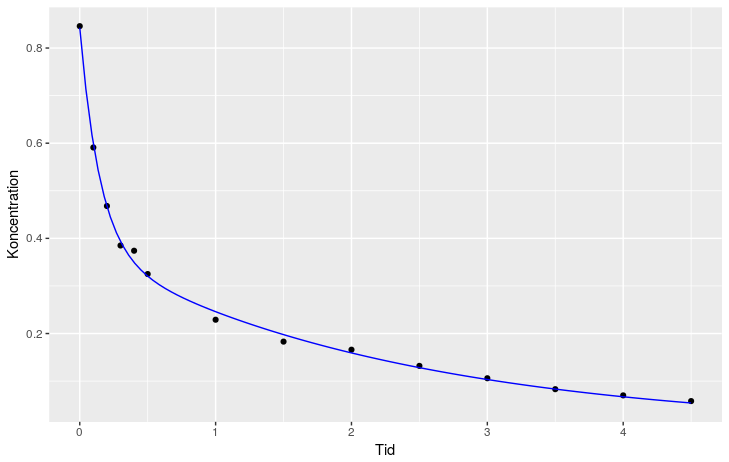
\includegraphics[scale=0.5]{q1p1.png}
\end{align}

\subsection{Delopgave g}

Fra de fundne udtryk for $A_1$ og $A_2$ i delopgave e får jeg disse to udtryk for $a_2$:
\begin{align}
a_2 = \frac{A_1(\lambda_1 - \lambda_2)}{K_{B0}} - \lambda_1 \\ \\
a_2 = \frac{A_2(\lambda_2 - \lambda_1)}{K_{B0}} - \lambda_2
\end{align}

Indsætter jeg $K_{B0}=0.846$ og de estimeterede værdier af $A_1, A_2, \lambda_1$ og $\lambda_2$ i disse udtryk får jeg $3.25$ og $3.92$ som estimater af $a_2$. Jeg estimerer derfor værdien af $a_2$ som gennemsnittet af disse to værdier, altså $3.586$.

Fra ligningen $\lambda_1\lambda_2 = a_2a_3$ fra delopgave b får jeg dette udtryk for $a_3$:
\begin{align}
a_3 = \frac{\lambda_1\lambda_2}{a_2}
\end{align}
Indsætter jeg de estimeterede værdier af $a_2, \lambda_1$ og $\lambda_2$ i dette udtryk, får jeg estimatet $a_3 = 0.812$. 

Fra ligningen $\lambda_1 + \lambda_2 = -a_1 - a_2 - a_3$ fra delopgave b, får jeg dette udtryk for $a_1$:
\begin{align}
a_1 = -\lambda_1 -\lambda_2 -a_2 -a_3
\end{align}
Indsætter jeg de estimeterede værdier af $a_2, a_3, \lambda_1$ og $\lambda_2$ i dette udtryk, får jeg estimatet $a_1 = 2.773$.

\subsection{Delopgave h}

I delopgave e bestemte jeg, at givet vores begyndeĺsesbetingelse får vi den partikulære model
\begin{align}
x(t) = \exp(\lambda_1 t)\frac{K_{B0}}{\lambda_1 - \lambda_2}\begin{pmatrix}
a_2 + \lambda_1\\
a_1
\end{pmatrix}  + \exp(\lambda_2t)\frac{K_{B0}}{\lambda_2 - \lambda_1}\begin{pmatrix}
a_2 + \lambda_2\\
a_1
\end{pmatrix}
\end{align}
Vi har nu estimater for alle konstanter i denne model. Indsætter vi dem, får vi følgende estimeterede model:
\begin{align}
x(t) = \exp(-0.432 t)\begin{pmatrix}
0.423\\
0.372
\end{pmatrix}  + \exp(-6.74t)\begin{pmatrix}
0.423\\
-0.372
\end{pmatrix}
\end{align}
Her er et plot over udviklingen af blods- og vævs-koncentrationen ifølge modellen
\begin{center}
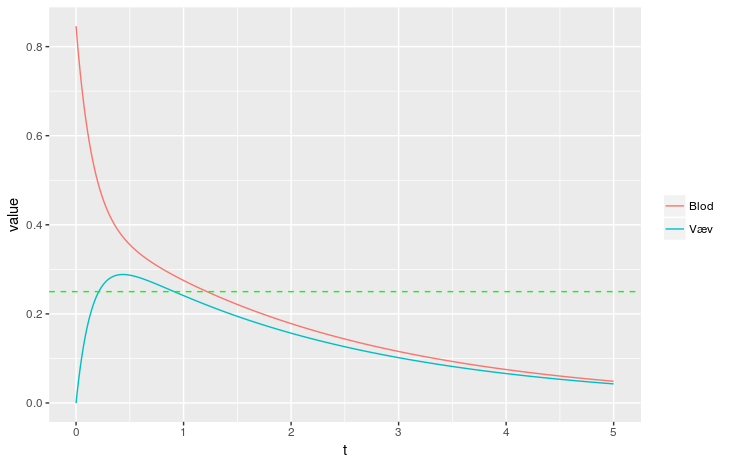
\includegraphics[scale=0.5]{q1p2.png}
\end{center}
Den grønne linje indikerer skæringen $y=0.25$. 

Ifølge modellen kan der opereres i tidsrummet mellem $t=0.21$ og $t=0.91$. Da $t$ er målt i timer, svarer det til, at man skal begynde, at operere efter
\begin{align}
0.21\text{time}\cdot 60 \frac{\min}{\text{time}} = 12.6\min
\end{align}
hvorefter der er et tidsrum på
\begin{align}
(0.91 \text{time} - 0.21\text{time})\cdot 60 \frac{\min}{\text{time}} = 42\min
\end{align}
til at nå operationen indenfor.

\subsection{Delopgave i}

Vi har nu systemet
\begin{align}
\begin{pmatrix}
K_B' \\ K_V'
\end{pmatrix} = f(K_B, K_V)
\end{align}
hvor 
\begin{align}
f(K_B, K_V) = \begin{bmatrix}
-(a_1 + a_3) & a_2 \\ 
a_1 & -a_2
\end{bmatrix}\begin{pmatrix}
K_B \\ K_V
\end{pmatrix} + \begin{pmatrix}
d_0 \\ 0
\end{pmatrix}
\end{align}

For at bestemme dets ligevægt løser jeg
\begin{align}
f(K_B^*, K_V^*) = (0,0)
\end{align}
hvorved jeg får
\begin{align}
\begin{pmatrix}
K_B^* \\ \\ K_V^*
\end{pmatrix} = \begin{pmatrix}
\frac{d_0a_1}{a_3} \\ \\ 
\frac{d_0a_2}{a_3}
\end{pmatrix}
\end{align}

Funktionalmatricen for $f$ er simpelthen
\begin{align}
Df(K_B, K_V) = \begin{bmatrix}
-(a_1 + a_3) & a_2 \\ 
a_1 & -a_2
\end{bmatrix}
\end{align}
Jeg har allerede vist i delopgave $b$, at denne matrix kun har egenværdier med negativ realdel, da jeg der viste, at den har to negative, reelle tal som egenværdier. Altså er den fundne ligevægt stabil.

\subsection{Delopgave j}

Da $K_V^*$ udtrykker koncentrationen af stoffet i vævet på lang sigt, skal jeg løse ligningen
\begin{align}
K_V^* = \frac{d_0a_2}{a_3} = 0.275
\end{align}
med hensyn til $d_0$. Hermed får jeg
\begin{align}
d_0 = \frac{a_3}{a_2} 0.275
\end{align}
Indsætter jeg de tidligere fundne estimater af $a_2$ og $a_3$ i dette udtryk, får jeg
\begin{align}
d_0 = 0.062
\end{align}

Jeg ved, at ligevægten $(K_B^*, K_V^*)$ er en partikulær løsning til det inhomogene system. Tidligere i opgaven fandt jeg den fuldstændige løsning til det homogene system. Altså kan jeg bestemme den fuldstændige løsning til det inhomogene system som summen af de to
\begin{align}
x(t) =   
c_1\exp(\lambda_1 t)\begin{pmatrix}
a_2 + \lambda_1\\
a_1
\end{pmatrix}  + c_2\exp(\lambda_2t)\begin{pmatrix}
a_2 + \lambda_2\\
a_1
\end{pmatrix} + \begin{pmatrix}
\frac{d_0a_1}{a_3} \\ 
\frac{d_0a_2}{a_3}
\end{pmatrix}
\end{align}

For at bestemme konstanterne i den ønskede partikulære løsning, vil jeg løse systemet
\begin{align}
\begin{pmatrix}
K_{B0} \\ 0
\end{pmatrix} =   
c_1\begin{pmatrix}
a_2 + \lambda_1\\
a_1
\end{pmatrix}  + c_2\begin{pmatrix}
a_2 + \lambda_2\\
a_1
\end{pmatrix} + \begin{pmatrix}
\frac{d_0a_1}{a_3} \\ 
\frac{d_0a_2}{a_3}
\end{pmatrix}
\end{align}
med hensyn til $c_1, c_2$, hvilket er ækvivalent med at løse systemet
\begin{align}
\begin{pmatrix}
K_{B0} - \frac{d_0a_1}{a_3} \\ - \frac{d_0a_2}{a_3}
\end{pmatrix} =  
\begin{bmatrix}
a_2 + \lambda_1 & a_2 + \lambda_2\\
a_1 & a_1
\end{bmatrix}
\begin{pmatrix}
c_1 \\ c_1
\end{pmatrix} 
\end{align}
der som bekendt har løsningen
\begin{align} 
\begin{pmatrix}
c_1 \\ c_1
\end{pmatrix} =
\begin{bmatrix}
a_2 + \lambda_1 & a_2 + \lambda_2\\
a_1 & a_1
\end{bmatrix}^{-1}
\begin{pmatrix}
K_{B0} - \frac{d_0a_1}{a_3} \\ - \frac{d_0a_2}{a_3}
\end{pmatrix} 
\end{align}
Jeg $K_{B0}=0.846$ og de estimeterede værdier af de andre størrelser i højresiden af dette udtryk. Hermed kan jeg få r til numerisk at bestemme værdien af det. Jeg får, at $c_1=0.051$ og $c_2=-0.15$. Jeg indsætter disse og de andre estimeterede værdier i udtrykket for den partikulære løsning, hvorefter jeg plotter udviklingen af koncentrationerne:
\begin{center}
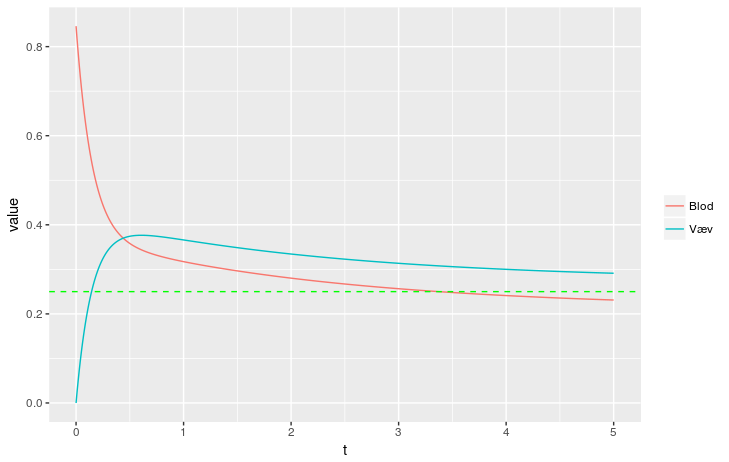
\includegraphics[scale=0.5]{q1p3.png}
\end{center}
Den grønne linje indikerer skæringen $y=0.25$. 

Ifølge modellen kan der opereres i tidsrummet efter $t=0.14$. Da $t$ er målt i timer, svarer det til, at man skal begynde, at operere efter
\begin{align}
0.14\text{time}\cdot 60 \frac{\min}{\text{time}} = 8.4\min
\end{align}
hvorefter der ikke er nogen tidsbegrænsning, da systemet konvergerer mod en ligevægt med vævskoncentration højere end $0.25$.

\section{Opgave 2}

For at bestemme systemets fulde fulde løsning, vil jeg bestemme egenværdierne til 
\begin{align}
A = \begin{bmatrix}
-2 & 1 \\
-4 & -2
\end{bmatrix}
\end{align}
Jeg udregner derfor det karakteristiske polynomien
\begin{align}
\det(A - \lambda E) = (-2 - \lambda)^2 + 4 = \lambda^2 + 4\lambda + 8
\end{align}
Diskriminanten for dette polynomien er
\begin{align}
d = 4^2 - 4\cdot 8 = -16
\end{align}
Polynomiets rødder er altså givet som
\begin{align}
\lambda_1 = \frac{-4 + \sqrt{-16}}{2} = -2 + 2i, \qquad \lambda_2=\lambda_1^* = -2 - 2i
\end{align}
For at bestemme en egenvektor til $\lambda_1$, løser jeg systemet
\begin{align}
(A - E\lambda)v = 0
\end{align}
hvilket giver mig egenrummet
\begin{align}
\{(v_1, v_2) \in \mathbb{C}^2 \ |\ v_1 = -2i v_2 \}
\end{align}
Fra dette egenrum vælger jeg egenvektoren
\begin{align}
q = \begin{pmatrix}
1 \\ -2i
\end{pmatrix}
\end{align}
Hermed får jeg også, at 
\begin{align}
q^* = \begin{pmatrix}
1 \\ 2i
\end{pmatrix}
\end{align}
er en egenvektor til egenværdien $\lambda_2$.

Altså kan jeg skrive den fuldstændige løsning for systemet op som
\begin{align}
\begin{pmatrix}
x(t) \\ y(t)
\end{pmatrix} = c_1\exp((-2+2i) t)\begin{pmatrix}
1 \\ -2i
\end{pmatrix} + c_2\exp((-2-2i) t)\begin{pmatrix}
1 \\ 2i
\end{pmatrix} 
\end{align}
hvor $c_1, c_2 \in \mathbb{C}$. 

Lad mig nu skrive denne løsning til reel form. Vi har, at 
\begin{align}
\exp((-2 + 2i)t)\begin{pmatrix}
1 \\ -2i
\end{pmatrix}  = \\ 
\exp(-2t)(\cos(2t) + i\sin(2t)) \begin{pmatrix}
1 \\ -2i
\end{pmatrix} = \\ 
\exp(-2t) \begin{pmatrix}
\cos(2t) + i\sin(2t) \\ -2i\cos(2t) + 2\sin(2t)
\end{pmatrix} = \\ 
\exp(-2t) \begin{pmatrix}
\cos(2t) \\ 2\sin(2t)
\end{pmatrix} + i\exp(-2t) \begin{pmatrix}
\sin(2t) \\ -2\cos(2t)
\end{pmatrix} 
\end{align}

Altså har vi, at
\begin{align}
Re\left(\exp((-2 + 2i)t)\begin{pmatrix}
1 \\ -2i
\end{pmatrix} \right) = \exp(-2t) \begin{pmatrix}
\cos(2t) \\ 2\sin(2t)
\end{pmatrix}
\end{align}
og
\begin{align}
Im\left(\exp((-2 + 2i)t)\begin{pmatrix}
1 \\ -2i
\end{pmatrix} \right) = \exp(-2t) \begin{pmatrix}
\sin(2t) \\ -2\cos(2t)
\end{pmatrix}
\end{align}

Altså har vi følgende fuldstændig løsning på reel form
\begin{align}
\begin{pmatrix}
x(t) \\ y(t)
\end{pmatrix} = b_1\exp(-2t) \begin{pmatrix}
\cos(2t) \\ 2\sin(2t)
\end{pmatrix} + b_2\exp(-2t) \begin{pmatrix}
\sin(2t) \\ -2\cos(2t)
\end{pmatrix}
\end{align}
hvor $b_1, b_2 \in \mathbb{R}$.

\subsection{Delopgave b}

For at bestemme den ønskede partikulære løsning, løser jeg systemet
\begin{align}
\begin{pmatrix}
3 \\ 4
\end{pmatrix} = b_1 \begin{pmatrix}
\cos(0) \\ 2\sin(0)
\end{pmatrix} + b_2 \begin{pmatrix}
\sin(0) \\ -2\cos(0)
\end{pmatrix} = b_1 \begin{pmatrix}
1 \\ 0
\end{pmatrix} + b_2 \begin{pmatrix}
0 \\ -2
\end{pmatrix}
\end{align}
hvilket giver $b_1=3$ og $b_2=-2$.

Her er et plot af udviklingen af $(x,y)$ som en kurve i planet:
\begin{center}
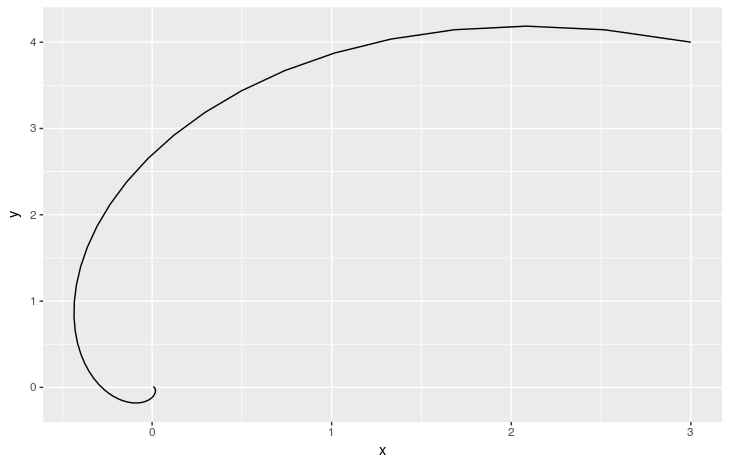
\includegraphics[scale=0.5]{q2p2.png}
\end{center}
og her er et plot med udviklingen af $x$ og $y$ hver for sig, plottet som funktioner af $t$:
\begin{center}
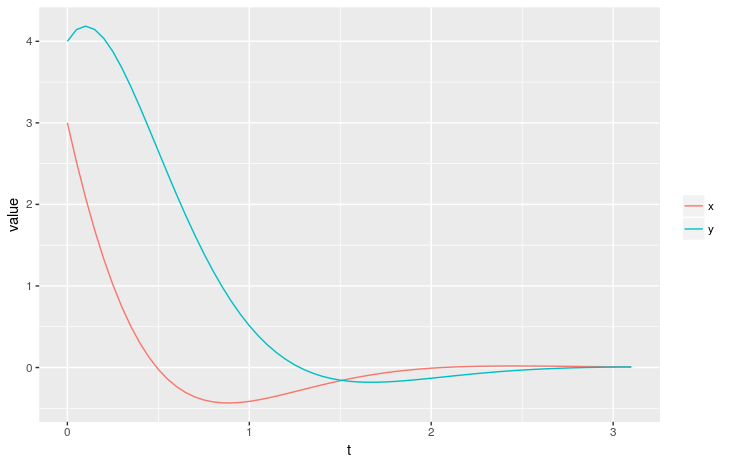
\includegraphics[scale=0.5]{q2p3.png}
\end{center}

\section{Delopgave c}

Jeg gætter på, at systemet har en løsning på formen
\begin{align}
\phi(t) = \begin{pmatrix}
k_1 \exp(2t) \\ k_2 \exp(2t)
\end{pmatrix}
\end{align}

Jeg indsætter dette i differentialligningen og får
\begin{align}
\phi'(t) = \begin{pmatrix}
2k_1 \exp(2t) \\ 2k_2 \exp(2t)
\end{pmatrix} = \begin{pmatrix}
-2k_1\exp(2t) + k_2\exp(2t) - \exp(2t) \\
-4k_1\exp(2t) - 2k_2\exp(2t) + 2\exp(2t)
\end{pmatrix}
\end{align}
hvilket er ækvivalent med
\begin{align}
\begin{pmatrix}
2k_1  \\ 2k_2 
\end{pmatrix} = \begin{pmatrix}
-2k_1 + k_2 - 1 \\
-4k_1 - 2k_2 + 2
\end{pmatrix}
\end{align}
hvilket er ækvivalent med
\begin{align}
\begin{pmatrix}
1  \\ -2 
\end{pmatrix} = \begin{bmatrix}
-4 & 1  \\
-4 & - 4
\end{bmatrix} \begin{pmatrix}
k_1 \\ k_2
\end{pmatrix}
\end{align}
hvilket giver $k_1=-0.1$ og $k_2=0.6$.

Jeg har nu fundet ud af, at 
\begin{align}
\phi(t) = \begin{pmatrix}
-0.1 \exp(2t) \\ 0.6 \exp(2t)
\end{pmatrix}
\end{align}
er en partikulær løsning til det inhomogene system. Jeg fandt den fuldstændige løsning til det homogene system ovenfor. Altså kan jeg bestemme den fuldstændige løsning til det inhomogene system som summen af de to
\begin{align}
\begin{pmatrix}
x(t) \\ y(t)
\end{pmatrix} = b_1\exp(-2t) \begin{pmatrix}
\cos(2t) \\ 2\sin(2t)
\end{pmatrix} + b_2\exp(-2t) \begin{pmatrix}
\sin(2t) \\ -2\cos(2t)
\end{pmatrix} + \begin{pmatrix}
-0.1 \exp(2t) \\ 0.6 \exp(2t)
\end{pmatrix}
\end{align}
hvor $b_1, b_2 \in \mathbb{R}$.

\section{Opgave 3}

\subsection{Delopgave a}

For at bestemme ligevægten, vil jeg løse systemet
\begin{align}
\begin{pmatrix}
0\\ 0
\end{pmatrix} = \begin{pmatrix}
-K_GW_S + K_DW_G + P_0 \\ 
Y_G K_G W_S - K_DW_G
\end{pmatrix}
\end{align}
Fra nederste ligning får jeg
\begin{align}
W_G = \frac{Y_GK_GW_S}{K_D}
\end{align}
hvilket jeg indsætter i øverste ligning, hvorved jeg får
\begin{align}
-K_GW_S + Y_GK_GW_S + P_0 = 0
\end{align}
hvilket giver mig
\begin{align}
W_S = \frac{P_0}{K_G(1 - Y_G)}
\end{align}
hvilket jeg indsætter tilbage i ovenstående udtryk for $W_G$, hvorved jeg får
\begin{align}
W_G = \frac{P_0Y_G}{K_D(1-Y_G)}
\end{align}
Hermed har jeg bestemt ligevægten
\begin{align}
\begin{pmatrix}
W_S^* \\ \\ W_G^*
\end{pmatrix} = \begin{pmatrix}
\frac{P_0}{K_G(1 - Y_G)} \\ \\
\frac{P_0Y_G}{K_D(1-Y_G)}
\end{pmatrix}
\end{align}

Funktionalmatricen for modellen er blot selve matricen, som har det karakteristiske polynomien
\begin{align}
(-K_G - \lambda)(-K_D - \lambda) - K_DY_GK_G = \lambda^2 + (K_G + K_D)\lambda + K_GK_D(1 - Y_G)
\end{align}
Da $0<K_D, K_G$ og $0<Y_G<1$, har vi altså, at det karakteristiske polynomien for funktionalmatricen er på formen
\begin{align}
\lambda^2 + A\lambda + B
\end{align}
hvor $A, B>0$. Altså har det kun rødder med negativ reaaldel. Altså har funktionalmatricen kun egenværdier med negativ realdel, og altså er ligevægten stabil.

\subsection{Delopgave b}

Ved hjælp af R bestemmer jeg, at modellens matrice har en egenværdien $\lambda_1=-2.32$ med tilhørende egenvektor 
\begin{align}
q_1 = \begin{pmatrix}
-0.777 \\ -0.069
\end{pmatrix}
\end{align}
og egenværdien $\lambda_2=-0.03$ med tilhørende egenvektor
\begin{align}
q_1 = \begin{pmatrix}
0.63 \\ -0.998
\end{pmatrix}
\end{align}

Alt i alt får jeg den fuldstændige løsning til
\begin{align}
x(t) = c_1\exp(-2.32t)\begin{pmatrix}
-0.777 \\ -0.069
\end{pmatrix} + c_2\exp(-0.03t)\begin{pmatrix}
0.63 \\ -0.998
\end{pmatrix} + \begin{pmatrix}
10.667 \\ 0.909
\end{pmatrix}
\end{align}

For begyndeĺsesbetingelsen $(W_S(0), W_G(0))=(2,10)$ finder jeg den partikulære løsning
\begin{align}
x(t) = 3.57\exp(-2.32t)\begin{pmatrix}
-0.777 \\ -0.069
\end{pmatrix} - 9.36\exp(-0.03t)\begin{pmatrix}
0.63 \\ -0.998
\end{pmatrix} + \begin{pmatrix}
10.667 \\ 0.909
\end{pmatrix}
\end{align}

Her er et plot af udviklingen af $W_S$ og $W_K$ over tid:
\begin{center}
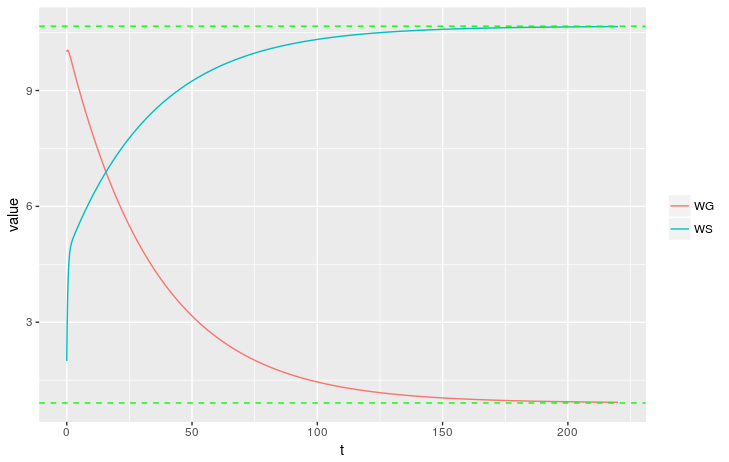
\includegraphics[scale=0.5]{q3p1.png}
\end{center}
De grønne linjer er ligevægtene.

\end{document}